\subsubsubsubsection{Active entity state}
\begin{figure}[h]
\centering
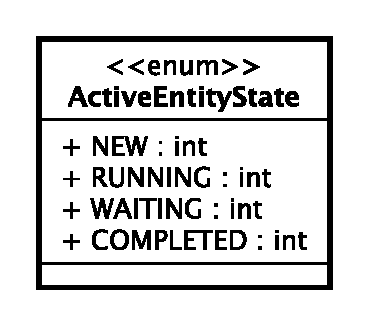
\includegraphics[scale=0.6,keepaspectratio]{images/solution/app/backend/active_entity_state.eps}
\caption{\pReactiveComponentStretchDecoration::ActiveEntityState}
\label{fig:sd-app-active-entity-state}
\end{figure}
\FloatBarrier
\begin{itemize}
  \item \textbf{\descr} \\
    It represents the state of an active entity.
  \item \textbf{\values}
  \begin{itemize}
    \item[+] \texttt{NEW: int} \\
    An active entity that has not yet started.
    \item[+] \texttt{RUNNING: int} \\
    An active entity that is executing an action.
    \item[+] \texttt{WAITING: int} \\
    An active entity that is waiting for executing a particular action.
    \item[+] \texttt{COMPLETED: int} \\
    An active entity that has completed its route.
  \end{itemize}
\end{itemize}